
\documentclass[xcolor=pdftex,dvipsnames,table,mathserif,aspectratio=169]{beamer}
\usetheme{default}
\usetheme{metropolis}
\usepackage{minted}
\usepackage{mathtools}
\setbeamersize{text margin left=.3in,text margin right=.3in} 

\DeclarePairedDelimiter\abs{\lvert}{\rvert}%
\DeclarePairedDelimiter\norm{\lVert}{\rVert}%


%\usetheme{Darmstadt}
%\usepackage{times}
%\usefonttheme{structurebold}

\usepackage[english]{babel}
%\usepackage[table]{xcolor}
\usepackage{pgf,pgfarrows,pgfnodes,pgfautomata,pgfheaps}
\usepackage{amsmath,amssymb,setspace,centernot}
\usepackage[latin1]{inputenc}
\usepackage[T1]{fontenc}
\usepackage{relsize}
\usepackage{pdfpages}
\usepackage[absolute,overlay]{textpos} 


\newenvironment{reference}[2]{% 
  \begin{textblock*}{\textwidth}(#1,#2) 
      \footnotesize\it\bgroup\color{red!50!black}}{\egroup\end{textblock*}} 

\DeclareMathSizes{10}{10}{6}{6} 

\begin{document}
\title{Part 8: Policy Evaluation\\
 Event Studies and Difference in Difference}
\author{Chris Conlon}
\institute{Applied Econometrics}
\date{\today}

\frame{\titlepage}

\begin{frame}{Motivation: Recap Matching}
Matching estimators had some advantages:
\begin{itemize}
\item Limited assumptions on \alert{functional forms}
\item We could do nearest neighbor matching and use kernels to compute treatment effects
\end{itemize}
Matching estimators had some drawbacks:
\begin{itemize}
\item Treated patients were ``matched'' to control patients based only on \alert{observable characteristics}
\begin{itemize}
\item Ignored \alert{selection on unobservables}.
\end{itemize}
\item Relied on \alert{cross sectional} variation to construct a control group.
\end{itemize}
\end{frame}


\begin{frame}{Motivation}
IV estimators resolve some of those issues but
\begin{itemize}
\item Good IV are in short supply!
\end{itemize}
 Often (in this course at least) we have access to \alert{panel data}.
\begin{itemize}
\item What if we could use panel data to control for \alert{unobserved heterogeneity} within a treated individual/group?
\end{itemize}
\alert{Difference in Difference} estimators are like the opposite of matching
\begin{itemize}
\item \alert{Strong} assumptions on \alert{functional form}
\item but... allow for \alert{unobservable heterogeneity} in outcomes.
\end{itemize}
\end{frame}


\section{A Famous Example: Card and Krueger (AER 1994)}

\begin{frame}{A Famous Example: Card and Krueger (AER 1994)}
\begin{itemize}
\item On April 1, 1992 NJ raises its minimum wage from $\$4.25\rightarrow \$5.05$ per hour.
\item Question: Econ 101 predicts this will \alert{reduce demand for low wage workers}
\begin{itemize}
\item Focus on fast food restaurants (since they pay min wage)
\item Focus on starting wage (avoid tenure, high turnover)
\end{itemize}
\item Survey 410 restaurants in NJ (treated group) and eastern PA (control group).
\item Idea: Compare \alert{change} in wages in $NJ$ to $PA$:  $\Delta_{DD} = \Delta_{NJ}- \Delta_{PA}$
\begin{itemize}
\item Wave 1: February 15-March 4, 1992
\item Wave 2: November 5 - December 31, 1992
\end{itemize}
\end{itemize}
\end{frame}

\begin{frame}{Balance Table: Covariates}
\begin{center}
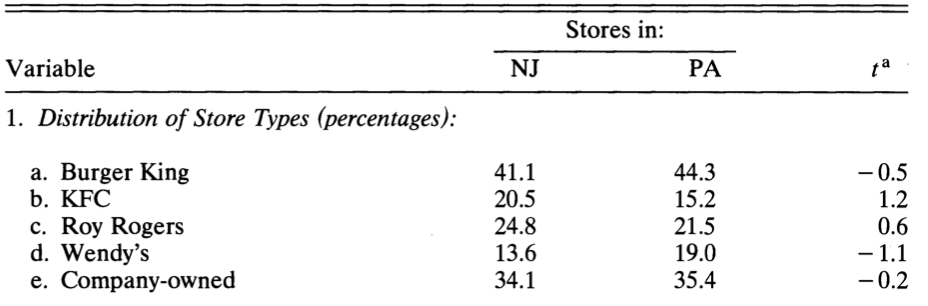
\includegraphics[width=2.25in]{./resources/ck_tab2b.png}\\
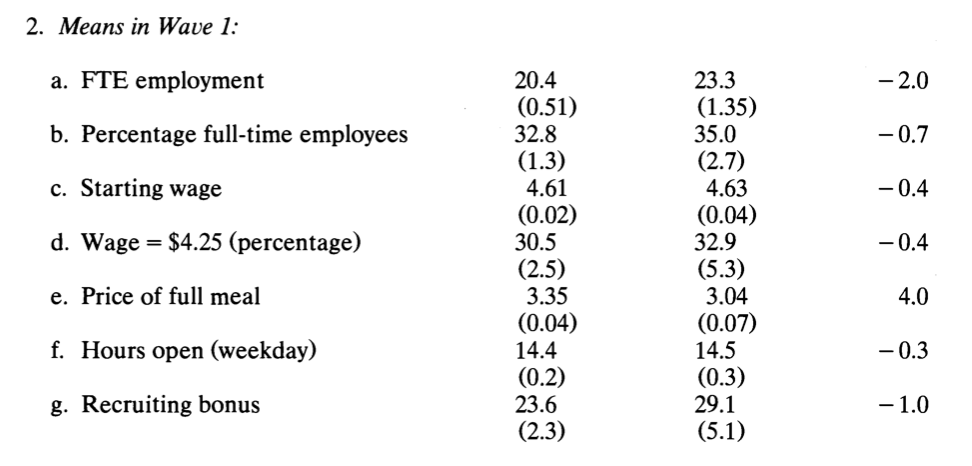
\includegraphics[width=2.25in]{./resources/ck_tab2c.png}\\
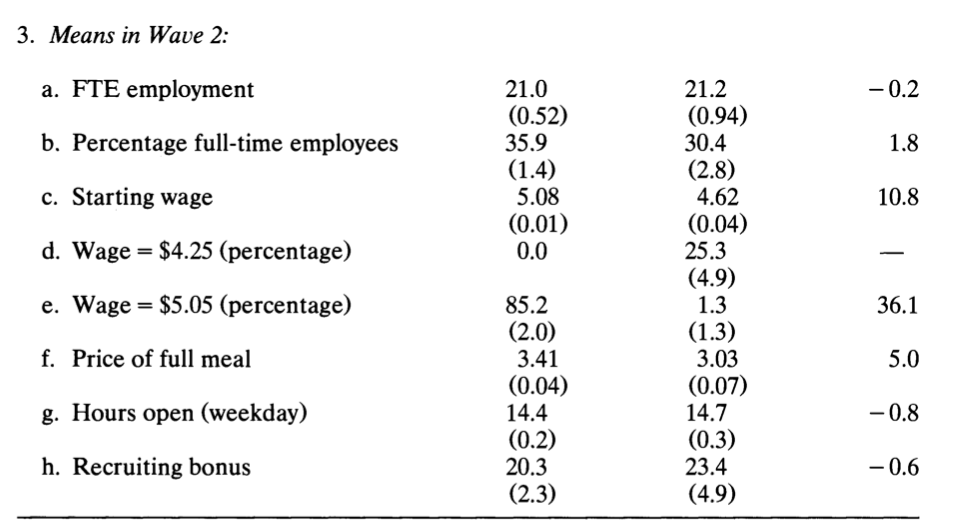
\includegraphics[width=2.25in]{./resources/ck_tab2a.png}
\end{center}
\end{frame}



\begin{frame}{Distribution of Wages}
\begin{center}
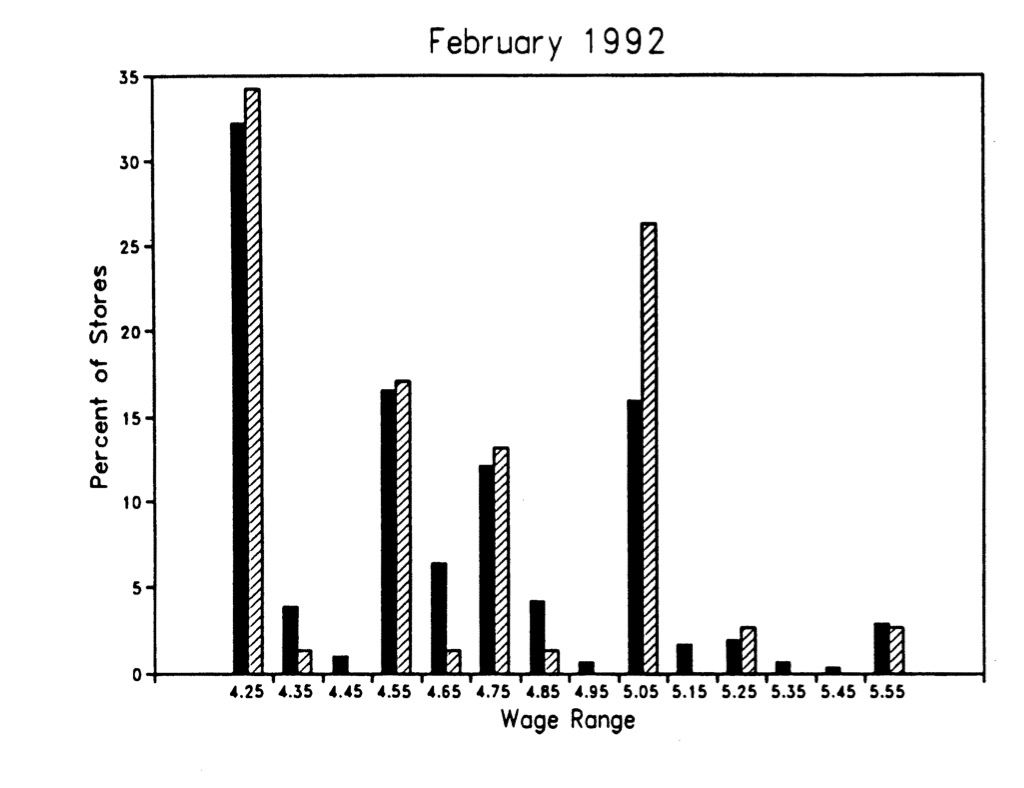
\includegraphics[width=2.75in]{./resources/ck_fig1b.png}
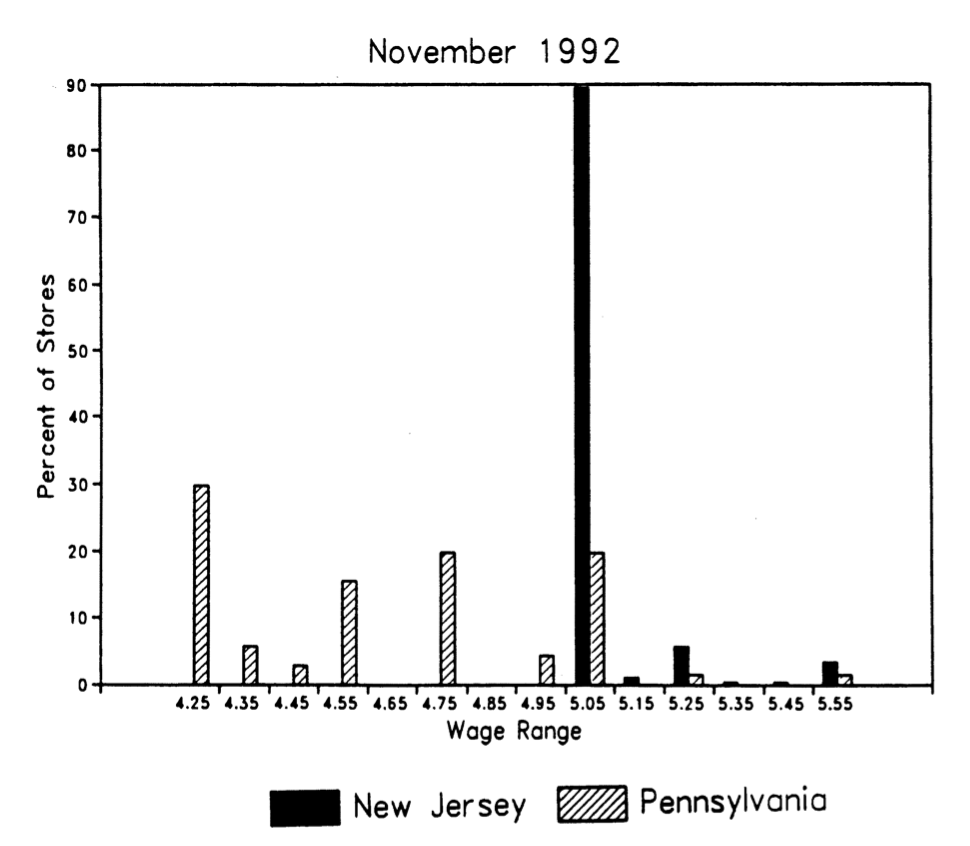
\includegraphics[width=2.5in]{./resources/ck_fig1a.png}
\end{center}
\end{frame}


\begin{frame}{Differences in Wages : 2 x 2 Table}
\begin{center}
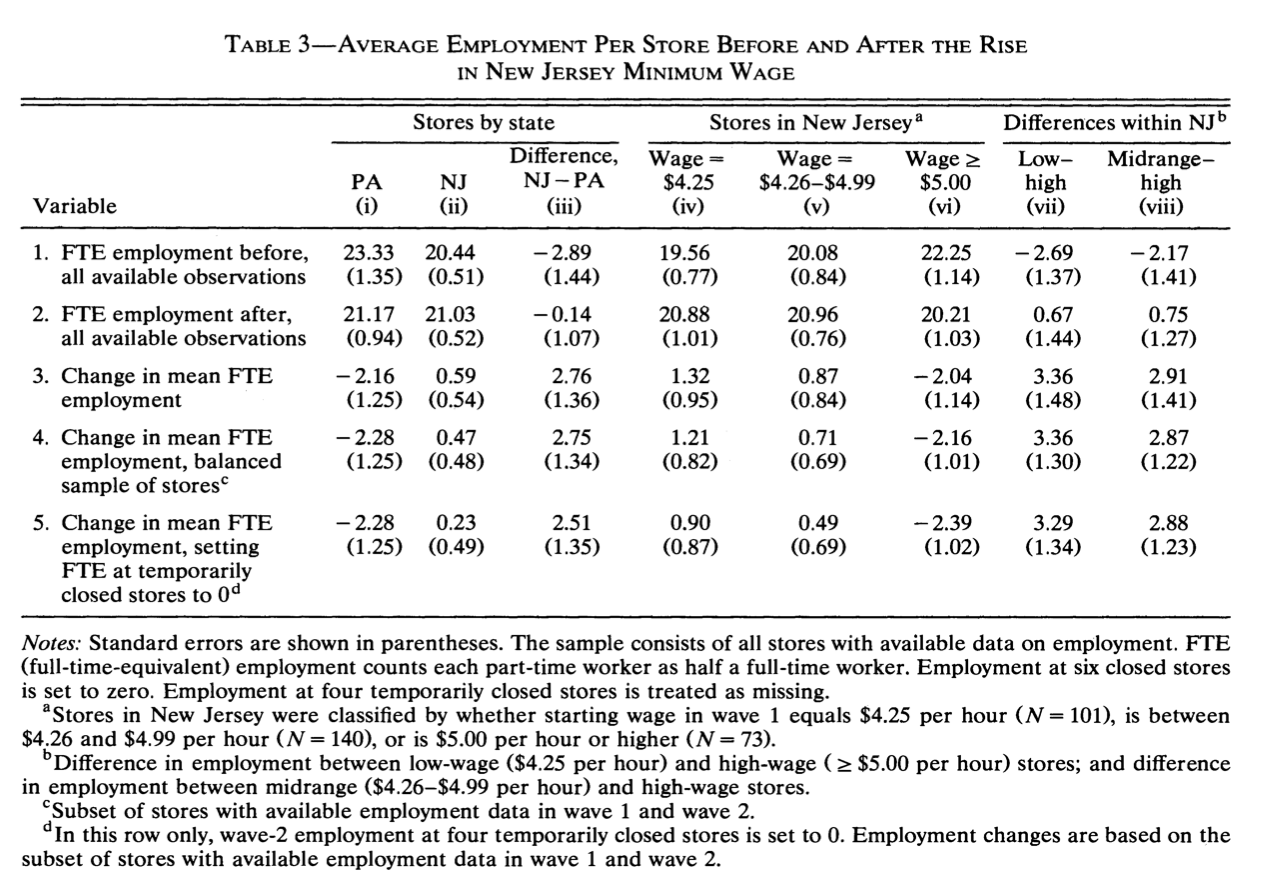
\includegraphics[width=4.25in]{./resources/ck_tab3.png}
\end{center}
\end{frame}

\begin{frame}{Outcome Equation}
\begin{itemize}
\item Differences lack any covariates (different fast food chains).
\item Also $\Delta_{PA}<0$ and $\Delta_{NJ} > 0$ (!)
\item Recall $i$ denotes stores, $t \in {1,2}$. Run the following regression:
\begin{align*}
Y_{it}&=\beta X_{it} +\alpha \cdot [i \in \text{NJ}] +  \gamma \cdot \text{After}_{t}  + \delta \cdot NJ_i \times After_{t} +u_{i}\\
Y_{it}&=\beta X_{it} +\alpha \cdot [\text{wage gap}_{i}] +  \gamma \cdot \text{After}_{t}  + \delta \cdot \text{wage gap}_{i} \times After_{t} +u_{i}
\end{align*}
\item $\alpha$ is mean difference between $NJ$ and $PA$
\item $\gamma$ is mean difference between period $1$ and $2$
\item $\delta$ is the parameter of interest, the \alert{difference in difference}
\item $\text{wage gap}_{i} = [\text{min wage}_{i,2}-w_{i1} ]_{+} =\max\{0, \text{min wage}_{i,2}-w_{i1}\} $.\\
 (How much do you need to raise $t=1$ wages to achieve minimum wage in $t=2$?)
\end{itemize}
\end{frame}

\begin{frame}{Differences in Wages}
\begin{center}
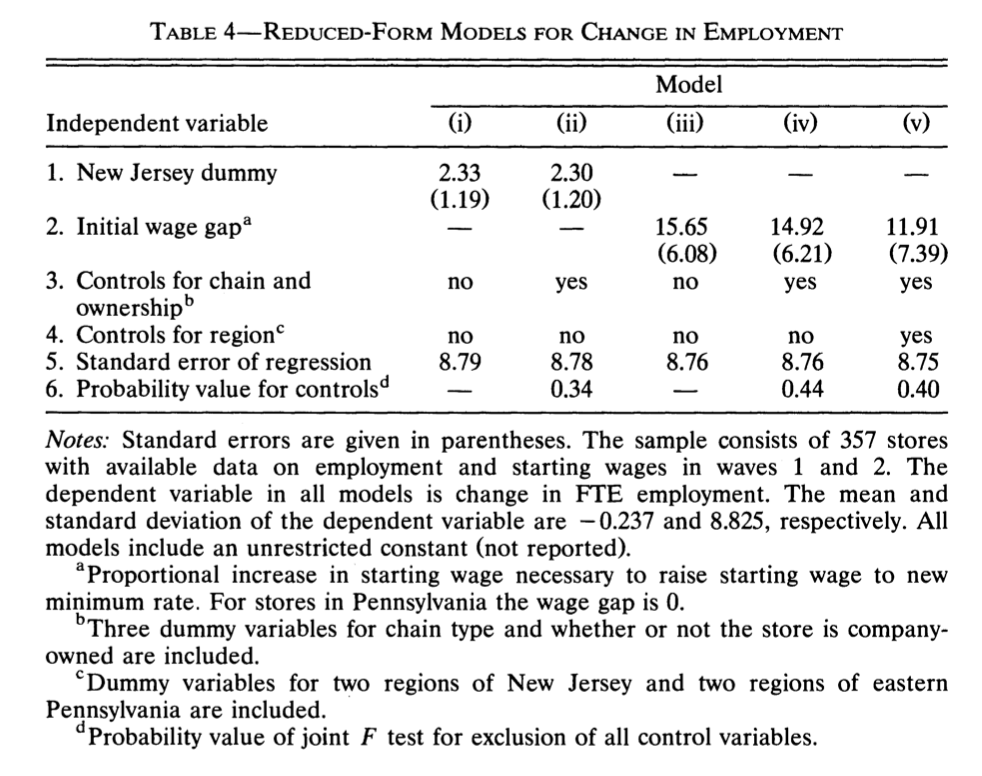
\includegraphics[width=4in]{./resources/ck_tab4.png}
\end{center}
\end{frame}

\begin{frame}{Before and After} 
For now let's not bother with a \alert{control group}.
\begin{itemize}
\item We look an outcome before or after an event $t \in {1,2}$
\begin{itemize}
\item $1$ \alert{before} event happens
\item $2$ \alert{after} event happens.
\end{itemize}

\begin{itemize}
\item A news event: the announcement of a merger or stock split.
\item A tax change, a new law, etc.
\end{itemize}
\item Except under strong conditions $d_2 = d_1$ we shouldn't believe the results of the before and after estimator.
\item Main Problem: we attribute changes to treatment that might have happened anyway \alert{trend}.
\item e.g: Cigarette consumption drops 4\% after a tax hike. (But it dropped 3\% the previous four years).
\item Also worry about: \alert{anticipation}, \alert{gradual rollout}, etc.
\end{itemize}
\end{frame}


\section{A More General Method}
\begin{frame}{General Case: Difference in Differences }
\begin{itemize}
\item Sometimes we may feel we can impose more structure on the problem.
\item Suppose in particular that we can write the outcome equation as
\begin{align*}
 Y_{it} =\alpha_i +\gamma_t +\delta_i T_{it}  + u_{it}
 \end{align*}
\item Suppose that $T_{i1}=0$ for all $i$ and $T_{i2}=1$ for a well defined group of individuals in our population.
\item This framework allows us to identify the ATT effect under the assumption that the growth of the outcome in the non-treatment state is independent of treatment allocation:
\begin{align*}
E[Y_{i2}(0) - Y_{i1}(0) | T_{i1}, T_{i2}] = E[Y_{i2}(0) - Y_{i1}(0)] 
\end{align*}
\item This is known as \alert{parallel trends}.
\end{itemize}
\end{frame}


\begin{frame}{Some Quick Algebra}
Recall our regression equation:
\begin{align*}
 Y_{it} =\alpha_i +\gamma_t +\delta_i T_{it}  + u_{it}
 \end{align*}
 This gives us:
\begin{align*}
E[Y_{i2} - Y_{i1} | T_{i2}=1] 
& = E[Y_{i2}(1) - Y_{i1}(1) | T_{i2}=1] \\
&= \underbrace{(\alpha_i - \alpha_i)}_{=0} + (\gamma_2-\gamma_1) + \underbrace{E[\delta_i  | T_{i2}=1]}_{ATT}  +  E[u_{i2} - u_{i1}  | T_{i2}=1] 
\end{align*}
\end{frame}






\begin{frame}{Difference in Differences} 
Let's try and estimate $d_2- d_1$ directly and then difference it out. Here we use \alert{parallel trends}:
\begin{align*}
E[Y_{i2}^0 - Y_{i1}^0 | T_{i2}=1]  &= E[Y_{i2}^0 - Y_{i1}^0 | T_{i2}=0] \\
E[Y_{i2} - Y_{i1} | T_{i2}=0] & = d_2-d_1
\end{align*}
We now obtain an estimator for ATT:
\begin{align*}
E[\beta_{i}| T_{i2}=1]  = E[Y_{i2} - Y_{i1} | T_{i2}=1] - E[Y_{i2} - Y_{i1} | T_{i2}=0]  
\end{align*}
which can be estimated by the difference in the growth between the treatment and the control group.
\end{frame}

\begin{frame}{Parallel Trends}
\begin{figure}
\centering
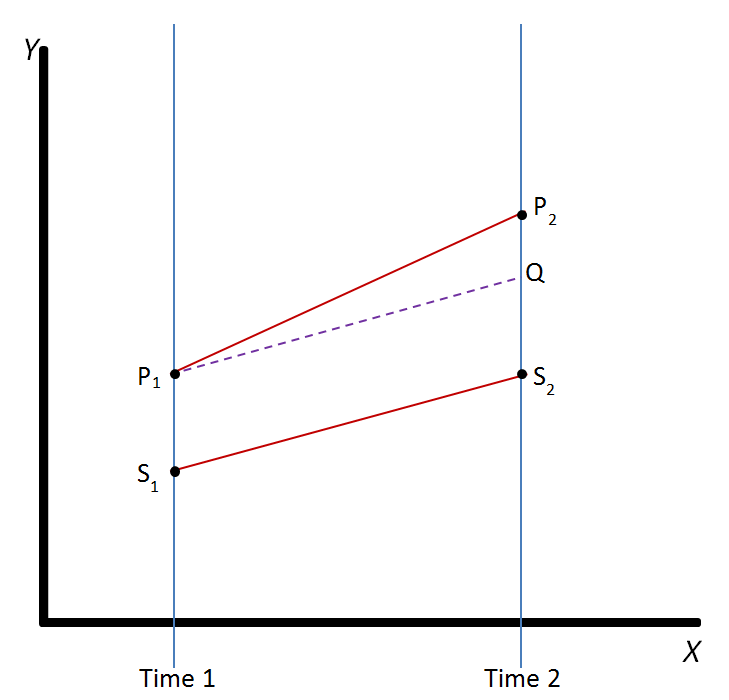
\includegraphics[width=3.5in]{./resources/parallel-trends}
\end{figure}
\end{frame}

\begin{frame}{Difference in Differences}
Now consider the following problem:
\begin{itemize}
\item Suppose we wish to evaluate a training program for those with low
earnings. Let the threshold for eligibility be $B$.
\item We have a panel of individuals and those with low earnings qualify for
training, forming the treatment group.
\item Those with higher earnings form the control group. 
\item Now the low earning group is low for two reasons
\begin{enumerate}
\item They have low permanent earnings ($\alpha_i$ is low) - this is accounted for by diff in diffs.
\item They have a negative transitory shock ($u_{i1}$ is low) - this is not accounted for by diff in diffs.
\end{enumerate} 
\end{itemize}
\end{frame} 

\begin{frame}{Difference in Differences}
\begin{itemize}
\item  \#2 above violates the assumption {\small $E[Y_{i2}^0 - Y_{i1}^0 | T] = E[Y_{i2}^0 - Y_{i1}^0]$}. 
\item To see why note that those participating into the program are such
that {\small $Y_{i0}^0 < B$}. Assume for simplicity that the shocks {\small $u$} are {\small $iid$}. Hence {\small $u_{i1} < B- \alpha_i - d_1$}. 
This implies: 
{\small $$E[Y_{i2}^0 - Y_{i1}^0 | T=1] = d_2 = d_1 - E[u_{i1}| u_{i1} <  B-\alpha_i - d_1]$$}
For the control group:
{\small $$E[Y_{i2}^0 - Y_{i1}^0 | T=1] = d_2 = d_1 - E[u_{i1}| u_{i1} >  B-\alpha_i - d_1]$$}
\item Hence
\begin{align*}
& E[Y_{i2}^0 - Y_{i1}^0 | T=1] - E[Y_{i2}^0 - Y_{i1}^0 | T=0] =\\
&  E[u_{i1} | u_{i1} >  B-\alpha_i - d_1] - E[u_{i1} | u_{i1} < B-\alpha_i - d_1]  >0
  \end{align*}
 \item This is effectively regression to the mean: those unlucky enough to have a bad shock recover and show greater growth relative to those with a good shock. The nature of the bias depends on the stochastic properties of the shocks and how individuals select into training.
\end{itemize}
\end{frame} 

\begin{frame}{Difference in Differences}
Ashefelter (1978) was one of the first to consider difference in differences to evaluate training programs.
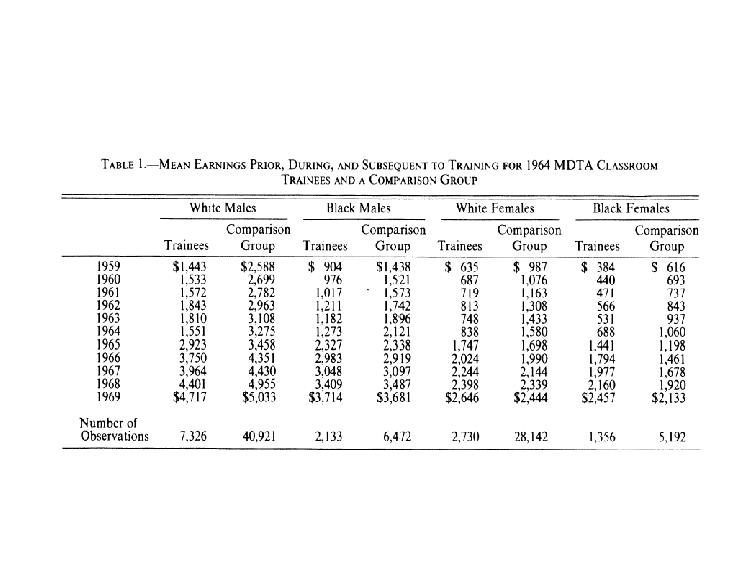
\includegraphics[scale=1]{./resources/ashefelter1.pdf}
\end{frame}

\begin{frame}{Difference in Differences}
Ashenfelter (1978) reports the following results.
\begin{figure}
\centering
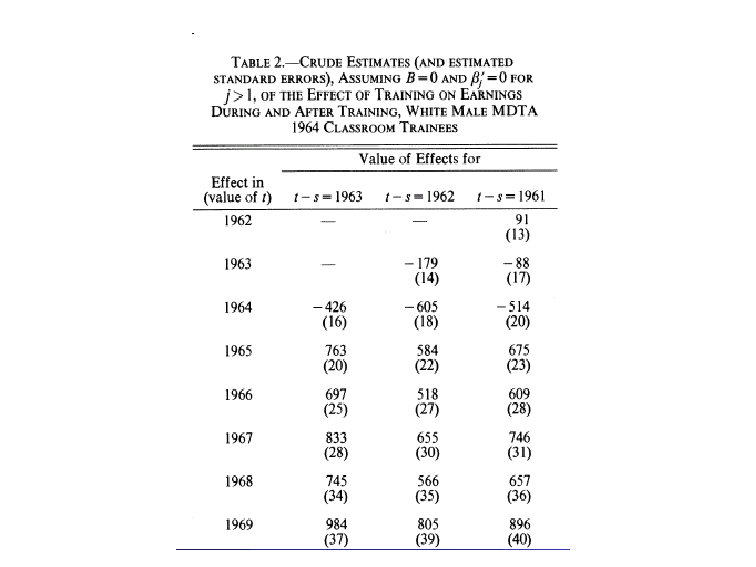
\includegraphics[scale=.85]{./resources/ashefelter2.pdf}
\end{figure}
\end{frame}

\begin{frame}{Difference in Differences}
\begin{itemize}
\item The assumption on growth of the non-treatment outcome being independent of assignment to treatment may be violated, but it may still be true conditional on $X$.
\item Consider the assumption
$$ E[Y_{i2}^0- Y_{i1}^0 | X,T] = E[Y_{i2}^0- Y_{i1}^0 | X] $$ 
\item This is just matching assumption on a redefined variable, namely the growth in the outcomes. In its simplest form the approach is implemented by running the regression
$$ Y_{it} = \alpha_i + d_t + \beta_i T_{it} + \gamma_t' X_i + u_{it}$$ 
which allows for differential trends in the non-treatment growth depending on $X_i$. More generally one can implement propensity score matching on the growth of outcome variable when panel data is available.
\end{itemize}
\end{frame}

\begin{frame}{Difference in Differences with Repeated Cross Sections}
\begin{itemize}
\item Suppose we do not have available panel data but just a random sample from the relevant population in a pre-treatment and a post-treatment period. We can still use difference in differences.
\item First consider a simple case where {\small $E[Y_{i2}^0- Y_{i1}^0 | T] = E[Y_{i2}^0- Y_{i1}^0]$}.
\item We need to modify slightly the assumption to
\vspace{-.5pc}
\begin{align*}
E[Y_{i2}^0| \text{\tiny Group receiving training}]&-E[Y_{i1}^0| \text{\tiny Group receiving training in the next period}] \\
&= E[Y_{i2}^0-Y_{i1}^0]  
\end{align*}
which requires, in addition to the original independence
assumption that conditioned on particular individuals that population we will be sampling from does not change composition.
\item We can then obtain immediately an estimator for ATT as
\begin{align*}
&E[\beta_i |T_{i2}=1] \\ 
&= E[Y_{i2}| \text{\tiny Group receiving training}]-E[Y_{i1}| \text{\tiny Group receiving training next period}] \\
&- \{E[Y_{i2} | \text{\tiny Non-trainees}] - E[Y_{i1} | \text{\tiny Group not receiving training next period}]\}
\end{align*}
\end{itemize}
\end{frame}


\begin{frame}{Difference in Differences with Repeated Cross Sections}
\begin{itemize}
\item More generalIy we need an assumption of conditional independence of the form
\begin{align*}
E[Y_{i2}^0 & | X, \text{\tiny Group receiving training}]-E[Y_{i1}^0| X, \text{\tiny Group receiving training next period}] \\
&= E[Y_{i2}^0 | X] - E[Y_{i1}^0 |X]
\end{align*}
\item Under this assumption (and some auxiliary parametric assumptions) we can obtain an estimate of the effect of treatment on the treated by the regression
\begin{align*}
Y_{it} = \alpha_g + d_t + \beta T_{it} + \gamma' X_{it} + u_{it}
\end{align*} 
\end{itemize}
\end{frame}

\begin{frame}{Difference in Differences with Repeated Cross Sections}
\begin{itemize}
\item More generalIy we can first run the regression 
\begin{align*}
Y_{it} = \alpha_g + d_t + \beta (X_{it}) T_{it} + \gamma' X_{it} + u_{it}
\end{align*} 
where $\alpha_g$ is a dummy for the treatment of comparison group, and $\beta (X_{it})$ can be parameterized as $\beta(X_{it}) = \beta' X_{it}$. The ATT can then be estimated as the average of $\beta' X_{it}$ over the (empirical) distribution of $X$.
\item A non parametric alternative is offered by Blundell, Dias, Meghir and van Reenen (2004).
\end{itemize}
\end{frame}

\begin{frame}{Difference in Differences and Selection on Unobservables}
\begin{itemize}
\item Suppose we relax the assumption of \emph{no selection} on unobservables. 
\item Instead we can start by assuming that
\begin{align*}
E[Y_{i2}^0 | X,Z] - E[Y_{i1}^0 | X,Z] = E[Y_{i2}^0 | X] - E[Y_{i1}^0 | X]
\end{align*} 
where $Z$ is an instrument which determines training eligibility say but does not determine outcomes in the non-training state. Take $Z$ as binary (1,0).
\item Non-Compliance: not all members of the eligible group ($Z = 1$) will take up training and some of those ineligible ($Z = 0$) may obtain training by other means.
\item A difference in differences approach based on grouping by $Z$ will estimate the impact of being allocated to the eligible group, but not the impact of training itself.
\end{itemize}
\end{frame}

\begin{frame}{Difference in Differences and Selection on Unobservables}
\begin{itemize}
\item Now suppose we still wish to estimate the impact of training on those being trained (rather than just the effect of being eligible)
\item This becomes an IV problem and following up from the discussion of LATE we need stronger assumptions
\begin{itemize}
\item  Independence: for $Z = a, \left\{Y_{i2}^0 - Y_{i1}^0, Y_{i2}^1 - Y_{i1}^1, T(Z=a)\right\}$ is independent of Z.
\item Monotonicity $T_i(1) \ge T_i(0) \, \forall \, i$
\end{itemize}
\item In this case LATE is defined by
 $$\left [E(\Delta Y | Z = 1) - E(\Delta Y | Z = 0)] / [Pr(T(1) = 1) - Pr(T(0) = 1) \right]$$
assuming that the probability of training in the first period is zero.
\end{itemize}              
\end{frame}



\end{document}

